\documentclass[12pt,a4paper,fleqn]{article}

\usepackage{ucs}
\usepackage[utf8x]{inputenc}
\usepackage[T2A]{fontenc}
\usepackage[english,russian]{babel}

\usepackage{textcomp}
\usepackage{indentfirst}
\usepackage{verbatim}
\usepackage{amsthm}
\usepackage{amssymb}
\usepackage{amsmath}
%\usepackage[colorlinks, urlcolor=blue, pdfborder={0 0 0 [0 0]}]{hyperref}
\usepackage{cmap}       % теперь из pdf можно копипастить русский текст
\usepackage{underscore} % Ура! Теперь можно писать подчёркивание.
\usepackage{graphicx}	% Пакет для включения рисунков

\usepackage[left=20mm,right=20mm,top=20mm,bottom=20mm]{geometry}

\IfFileExists{cyrtimes.sty}
{
  \usepackage{cyrtimespatched}
} 
{
  % А если Times нету, то будет CM...
}

\usepackage{color}

\usepackage{listings}
% Значения по умолчанию для listings
\lstset{
  basicstyle=\footnotesize,
  frame=none,
  breakatwhitespace=true,% разрыв строк только на whitespacce
  breaklines=true,       % переносить длинные строки
  captionpos=b,          % подписи снизу
  numbers=none,          % без нумерации
  showspaces=false,      % показывать пробелы подчеркиваниями -- идиотизм 70-х годов
  showstringspaces=false,
  showtabs=false,        % и табы тоже
  stepnumber=1,
  tabsize=4              % кому нужны табы по 8 символов?..
}

% Стиль для псесдовода: строчки обычно короткие, поэтому размер шрифта побольше
\lstdefinestyle{pseudocode}{
  basicstyle=\small,
  frame=none,
  keywordstyle=\color{black}\bfseries\underbar,
  language=Pseudocode,
  numberstyle=\footnotesize,
  commentstyle=\footnotesize\it
}

% Стиль для обычного кода: маленький шрифт
\lstdefinestyle{realcode}{
  basicstyle=\scriptsize,
  frame=none,
  numberstyle=\footnotesize
}

% Стиль для коротких кусков обычного кода: средний шрифт
\lstdefinestyle{simplecode}{
  basicstyle=\footnotesize,
  frame=none,
  numberstyle=\footnotesize
}

% Определим свой язык для написания псевдокодов на основе Python
\lstdefinelanguage[]{Pseudocode}[]{Python}{
  morekeywords={each,empty,wait,do},% ключевые слова добавлять сюда
  morecomment=[s]{\{}{\}},% комменты {а-ля Pascal} смотрятся нагляднее
  literate=% а сюда добавлять операторы, которые хотите отображать как мат. символы
    {->}{\ensuremath{$\rightarrow$}~}2%
    {<-}{\ensuremath{$\leftarrow$}~}2%
    {:=}{\ensuremath{$\leftarrow$}~}2%
    {<--}{\ensuremath{$\Longleftarrow$}~}2%
}[keywords,comments]

\sloppy
\hyphenpenalty=9000

\makeatletter
\renewcommand\@biblabel[1]{\hfill#1.}
\makeatother

\newcommand\regsign{\textsuperscript{\textcircled{\scriptsize{R}}}}
\newcommand\copysign{\textsuperscript{\copyright}}
\newcommand\tmsign{\textsuperscript{\scriptsize{TM}}}

\newcommand{\Code}[1]{\textbf{\mbox{#1}}}
\newcommand{\Term}[1]{\emph{\mbox{#1}}}

\usepackage{alltt}

\newenvironment{CodeBlock}{\begin{alltt}\small}{\end{alltt}}

\DeclareMathOperator*{\StateTransN}{\Rightarrow}
\DeclareMathOperator{\StateTrans}{\StateTransN^T}

\newcommand\etc{~и~т.д.}
\newcommand\etca{~и~т.п.}

\title{Описание заявки на конкурс HPC Contest 2010: Parallel Spin}
\author{Коротков\,И.\,А.}

\begin{document}

  % a.. описание задачи; 
  % b.. требования к вычислительным ресурсам при ее решении в настоящее время; имеющиеся подходы к решению (уже разработанные); 
  % c.. суть предлагаемого проекта - что сделано/будет сделано в результате проекта; 
  % d.. сравнение с имеющимися подходами и преимущества; 
  % e.. обоснование необходимости и эффективности применения суперкомпьютеров для расчетов в предлагаемых для конкурса проектах; 
  % f.. описание методов, с помощью которых достигается эта эффективность; 
  % g.. перспективы использования, ожидаемая эффективность от внедрения приложения, практическое применение, потенциальные потребители. 

\section{Описание задачи}

При разработке сложных параллельных систем (систем, состоящих из нескольких асинхронно
работающих компонент) с высокой степенью надежности традиционных подходов к тестированию
зачастую бывает недостаточно, поскольку они позволяет выявить лишь легко воспроизводимые
ошибки. В некоторых случаях, например, в программном обеспечении для бортовых систем,
определенные классы ошибок требуется полностью исключить.

Для таких случаев применяется проверка модели (model checking)~--- автоматический
формальный подход, при котором на основе дискретной детерминированной модели программы или
комплекса программ строится полное пространство состояний и на нем проверяется набор
интересующих нас утверждений~--- спецификация. Проверку моделей можно использовать для
поиска взаимоблокировок в параллельных алгоритмах и ошибок в спецификациях сетевых
протоколов. В качестве примера можно привести протокол маршрутизации RIP: проверка модели
сети из четырех маршрутизаторов, соединенных четыремя сетевыми интерфейсами, на предмет
возникновения циклов в маршрутных таблицах позволяет убедиться, что существуют сценарии,
при которых такие циклы возникают, и необходимо использование специальных мер
(расщепленный горизонт) для их избежания.

Наиболее распространенным средством проверки конечных моделей является ПО SPIN,
использующее для описания исходной модели язык \emph{Promela} (PROtocol Meta Language).

Модель на языке Promela описывается в виде набора процессов, состоящих из последовательности
команд. Каждый процесс имеет свой набор локальных переменных (в том числе счетчик команд). Для
взаимодействия между процессами могут использоваться глобальные переменные и каналы (очереди
сообщений). Каждая команда имеет свое условие выполнимости, и процесс считается заблокированным,
если условие выполнимости его текущей команды не выполнено.

Пример описания модели семафора Дейкстры и трех захватывающих его процессов в нотации
Promela привен ниже:

\begin{lstlisting}[language=Promela]
mtype { p, v };
chan sema = [0] of { mtype };
active proctype Dijkstra()
{      byte count = 1;
       do
       :: (count == 1) ->
               sema!p; count--
       :: (count == 0) ->
               sema?v; count++
       od
}
active [3] proctype user()
{       do
        :: enter: sema?p;  /* enter critical section */
            crit: skip;    /* critical section */
                  sema!v;  /* leave critical section */
        od
}  
\end{lstlisting}

В ходе верификации SPIN выполняет исчерпывающий поиск в глубину по графу состояний и, при
обнаружении пути, на котором нарушается проверяемое утверждение, сохраняет его в качестве
контрпримера. Если контрпример обнаружить не удается, верификация успешна.

Spin принимает в качестве входных данных модель многопоточной системы на языке Promela и
генерирует файл с кодом на языке С. Полученный код выполняет исчерпывающий поиск по
пространству состояний $S$ в глубину, добавляя посещенные состояния в хэш-таблицу, что
можно представить следующим псевдокодом:

\begin{lstlisting}[style=pseudocode]
Visited = []

def StateSpaceDFS(state):
    if not state in Visited:
        Visited <- state
        for each new_state in Next(state):
            StateSpaceDFS(new_state)

StateSpaceDFS(initial_state)
\end{lstlisting}

При генерации каждого состояния делается проверка, было ли оно уже посещено ранее (т.е. находится в
множестве \Code{Visited}) и добавление в этом множество в противном случае.

\section{Требования к вычислительным ресурсам}

Последовательное построение пространства состояний $S$ с ростом размера модели быстро
становится невозможным из-за нехватки памяти для хранения множества достигнутых состояний
(\Code{Visited}). В табл.~\ref{tab:models-statecount} приведены данные для двух моделей:
модели задачи об обедающих философов и более приближенной к реальным задачам модели
RIP-протокола на 4 сетевых маршрутизаторах.

\begin{table}
  \centering
  \begin{tabular}{|r|l|l|}
    \hline
    Модель                  & Состояний         & Переходов       \\
    \hline
    Философы (5)            & $2.8 \cdot 10^4$  & $4.2 \cdot 10^4$ \\
    Философы (7)            & $3.6 \cdot 10^5$  & $6.0 \cdot 10^5$ \\
    RIP (4 маршрутизатора)  & $1.6 \cdot 10^8$  & $4.8 \cdot 10^9$ \\
    \hline
  \end{tabular}
  \caption{Количество состояний и переходов в различных моделях}
\label{tab:models-statecount}
\end{table}

Из табл. \ref{tab:models-statecount} видно, что для реальных моделей традиционный подход
становится проблематичен: к примеру, модель RIP-протокола с 5-ю маршрутизаторами потребует
уже более 100 Гб оперативной памяти для хранения пространства состояний.

\section{Существующие подходы к решению задачи}

Существует ряд подходов, решающих данную проблему. Среди них можно выделить:

\begin{itemize}
\item методы оптимизации, уменьшающие количество хранимых состояний;
\item методы оптимизации, уменьшающие расход памяти на их хранение;
\end{itemize}

\textbf{Сокращение частных порядков} (\Term{partial order reduction}) относится к первой
группе: оно уменьшает количество генерируемых состояний. Данный метод использует тот факт,
что зачастую порядок выполнения двух переходов в различных процессах не оказывает влияния
на результат проверки, поэтому в случае двух независимых переходов, не меняющих
проверяемых свойств системы, генерируется лишь одна последовательность!!!

При \textbf{битовом хэшировании состояний} (\Term{bit-state hashing}) вместо традиционной
хэш-таблицы для хранения состояний используется битовая таблица. Каждое состояние $s$
представлено в ней битом с номером $i = hash(s)$. Нулевой бит означает, что состояние еще
не было достигнуто, единичный — было. При этом вся используемая память отводится под
хэш-таблицу (сами состояния не хранятся). При размере состояния в 20-30 байт это позволяет
хранить в 160-240 больше состояний, чем при традиционном подходе.

Однако, коллизии в этом случае обнаружить невозможно -- состояния будут просто
<<теряться>>, поэтому приходится просто полагаться на то, что коллизий не возникнет (для
этого надо обеспечить низкую степень заполненности таблицы) или что <<потерянные>>
состояния не повлияют на итог.

\textbf{Сжатие состояние}, например, с использованием кодов Хаффмана, позволяет уменьшить требуемый
объем памяти в 4--5 раз за счет увеличения времени проверки.

Приведенные меры либо дают небольшой, плохо масштабируемый прирост, либо приводят к потенциальным потерям
состояний при обходе.

\section{Предлагаемый подход}

Альтернативным подходом является \emph{параллельная генерация состояний} с распределенным хранением
по различным узлам вычислительной сети.

Каждый узел является одновременно хранилищем и генератором и хранит очередь состояний
$Q$. Порождая новое состояние, узел $i$ проверяет, какому узлу оно принадлежит; если это
узел $j$, не совпадающий с данным ($i \neq j$), $i$ делает удаленный вызов $j$, в
результате которого состояние добавляется в очередь $Q_j$. Если состояние принадлежит тому
же узлу ($j = i$), он проверяет, не входит ли оно в множество посещенных состояний
\Code{Visited} и добавляет его в свою очередь $Q_i$. При этом каждый узел выполняет что-то
вроде поиска в ширину, однако какой-либо глобальный порядок обхода отсутствует~--- он не
соответствует ни обходу в ширину, ни обходу в глубину.

Порядок генерации того же набора состояний, что и в предыдущем примере, показан на
рис.~\ref{fig:distr-generation}.

\begin{figure}[!htb]
  \centering
  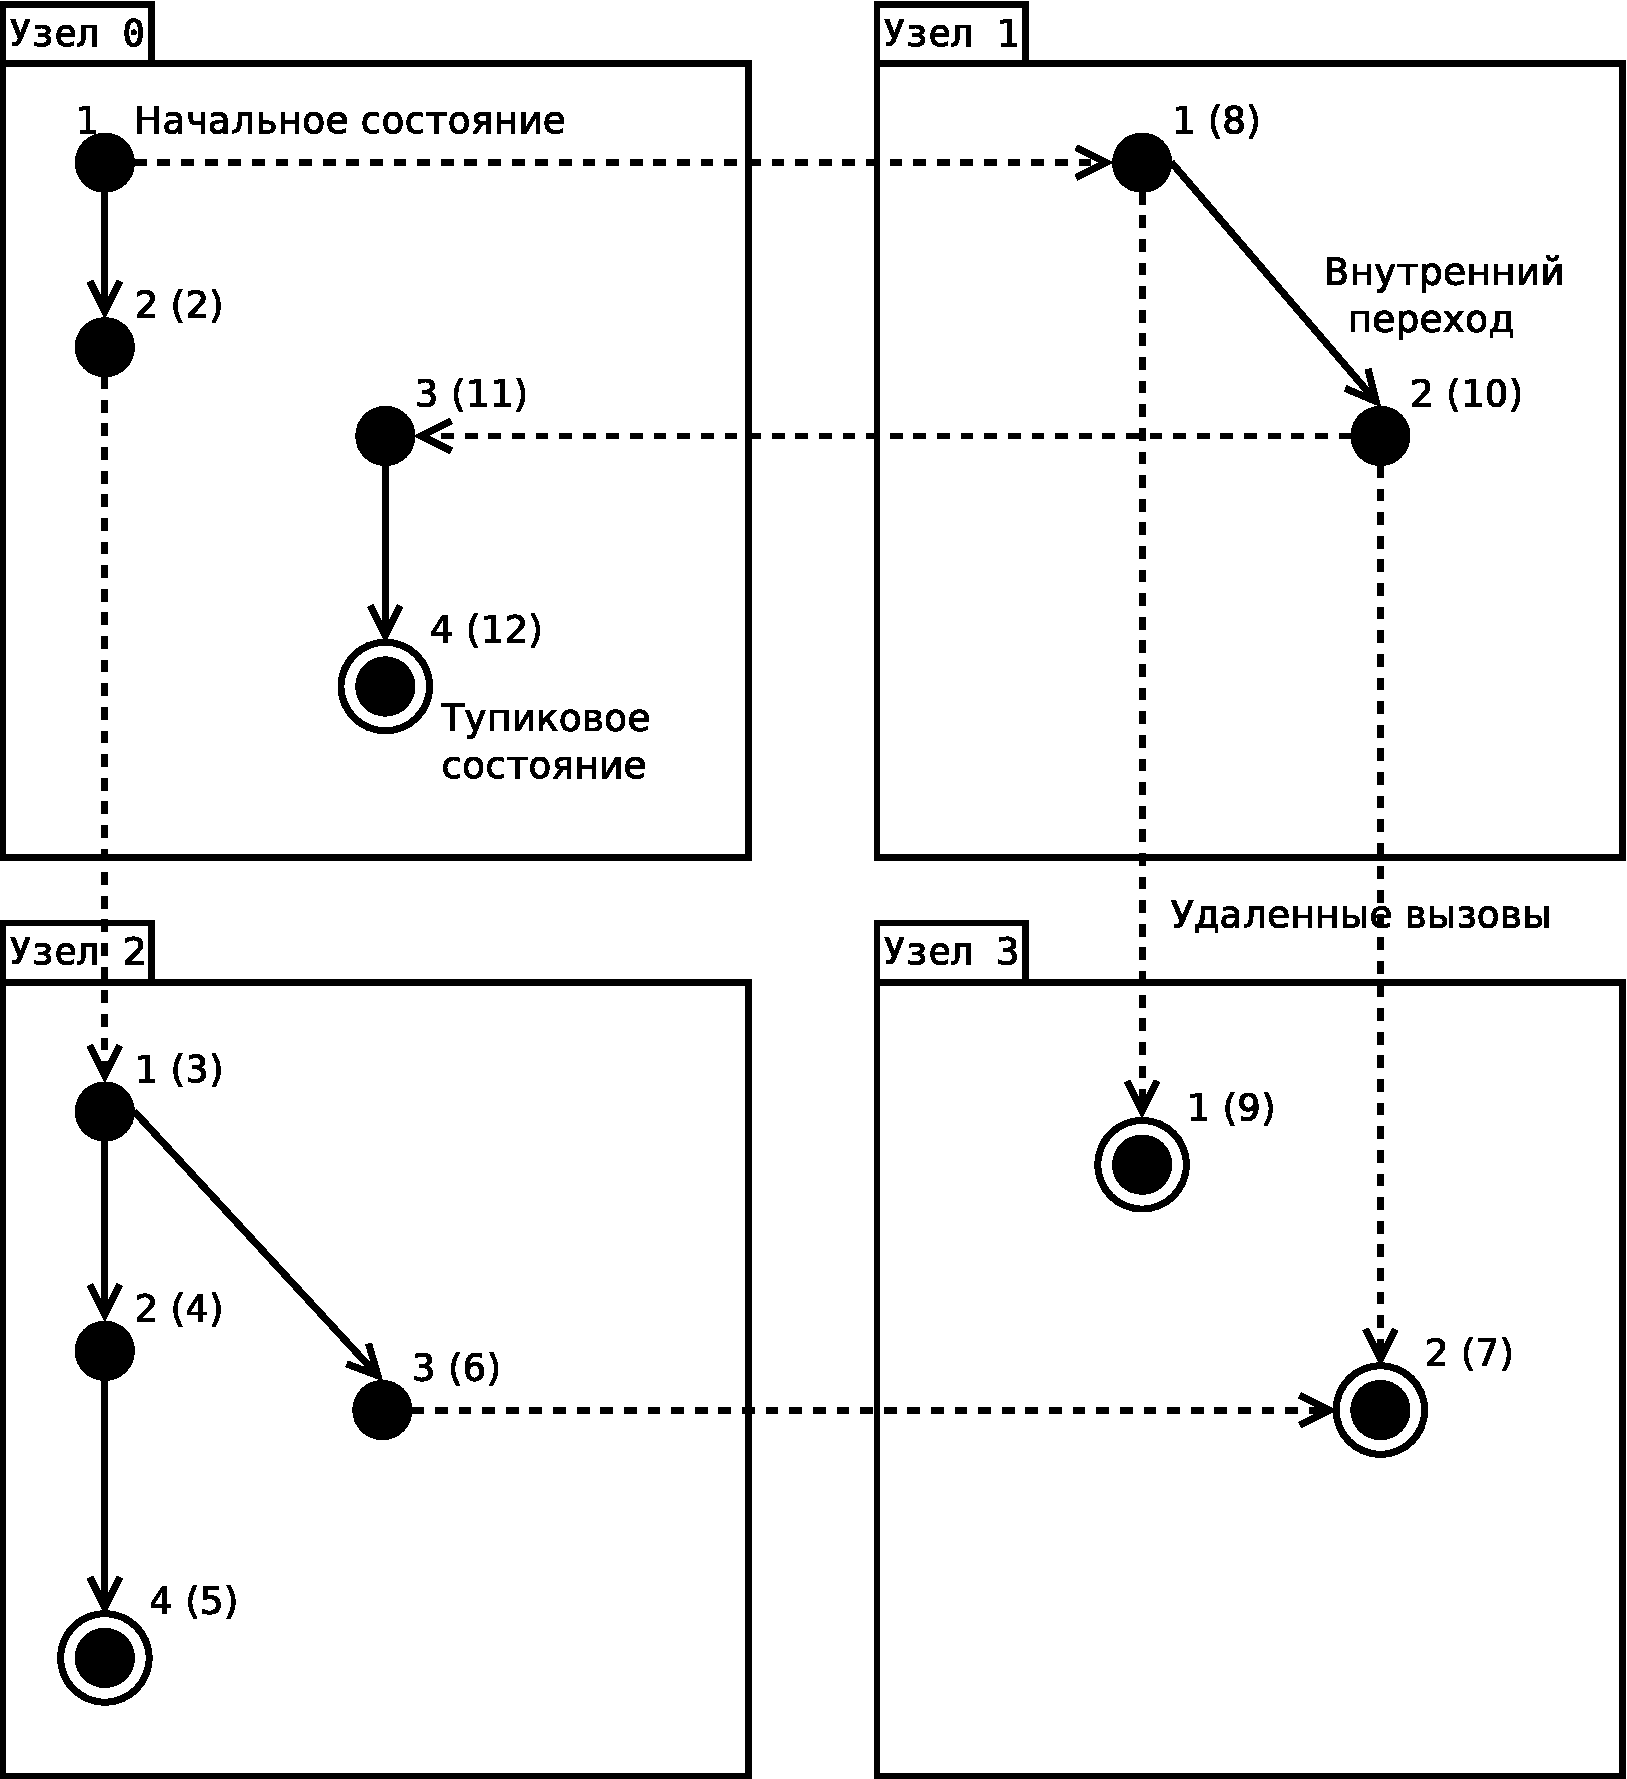
\includegraphics[width=0.75\textwidth]{../graphics/distr-generation}
  \caption{Пример работы алгоритма распределенной генерации}
  \label{fig:distr-generation}
\end{figure}

Псевдокод, выполняемый на всех узлах:

\begin{lstlisting}[style=pseudocode]
Visited = []
Queue   = [initial_state]

def ParStateSpaceBFS():
    while not empty(Queue):
        Queue -> state
        node = StateNode(state)
        if NodeId = node:
            if not state in Visited:
                Visited <- state
                for each new_state in Next(state):
                    Queue <- new_state
        else:
            node.Queue <- state

ParStateSpaceBFS()
\end{lstlisting}

Здесь \Code{node.Queue $\leftarrow$ state}~--- удаленный вызов, добавляющий состояние в очередь узла
\Code{node}.

В приведенном коде для определения номера узла, хранящего сообщения, используется функция
\Code{StateNode}. Эта функция должна обладать следующими свойствами:

\begin{itemize}
\item она должна зависеть только от битового представления самого состояния, поскольку одно и то же состояние
  может генерироваться различными узлами в результате различных переходов;

\item она должна распределять состояния между узлами достаточно равномерно, в противном случае часть памяти у некоторых
  узлов будет простаивать;

\item она должна обладать свойством локальности относительно переходов между состояниями~--- по возможности новые
  состояния должны принадлежать тому же узлу, что и исходное.
\end{itemize}

Можно использовать в качестве \Code{StateNode} хэш-функцию от битового представления
состояния $s$: это обеспечит первые два условия, но третье (локальность) нарушается, что
приведет к частым удаленным вызовам между узлами.

Битовое представление состояния в общем случае представляет собой набор значений
переменных, описывающих состояние отдельных компонент (локальные переменные процессов в
нотации Promela) моделируемой системы и значения глобальных переменных, описывающих
взаимодействие между ними.

Для соблюдения условия локальности в качестве \Code{StateNode} используется хэш-функция не
от всего состояния, а от локального состояния первых нескольких (одного или двух)
процессов (в нотации Promela).

Подсчеты показывает, что при количестве процессов $P = 6-8$, при распределении по хэшу
первого процесса получается в 4--5 раз меньше удаленных вызовов, чем при хэшировании
состояния целиком.

\section{Организация хранения состояний}

Каждый узел хранит множество посещенных состояний \Code{Visited}, текущую очередь \Code{Queue} и
хэш-таблицу для быстрого поиска состояний в \Code{Visited}. В зависимости от того, какой тип
хэширования выбран, состояния хранятся в них по-разному.

В данной работе рассматриваются два подхода: полное хэширование с открытой адресацией и
битовое хэширование с произвольным (задаваемым) число хэш-функций.

\subsection{Полное хэширование}

При полном хэшировании хэш-таблица хранит указатели на состояния в \Code{Visited}. Сами
состояния хранятся при этом отдельно, это связано с тем, что их размер заранее не
определен и может меняться, тогда как записи в таблице должны быть фиксированного размера.

Для того, чтобы избежать ненужного копирования, множество посещенных состояний \Code{Visited}
объединяется с \Code{Queue}. Новое состояние проверяется на вхождение в хэш-таблицу сразу при
генерации, и в случае отсутствия добавляется в \Code{Queue}. Таким образом, все попадающие в
\Code{Queue} состояния рано или поздно перейдут в \Code{Visited}, поэтому они занимают один
последовательный блок памяти, как это показано на рис.~\ref{fig:fullstate}. Новые состояния
добавляются в верхнюю часть \Code{Queue}, при этом указатель на начало свободной области сдвигается
вверх. Выборка состояний из \Code{Queue} делается с низу очереди, при этом указатель на ее начало
сдвигается (и состояние <<переносится>> в \Code{Visited}). Если свободная область памяти
заканчивается, алгоритм завершается с ошибкой.

\begin{figure}[ht]
  \centering
  \includegraphics[width=1\textwidth]{../graphics/fullstate}
  \caption{Хранение состояний при полном хэшировании}
  \label{fig:fullstate}
\end{figure}

\subsection{Битовое хэширование}
\label{sec:bithash-store}

При битовом хэшировании состояния после добавления в хэш-таблицу отбрасываются и занимаемая ими
память используется для хранения следующих состояний. Поэтому множество \Code{Visited} как таковое
отсутствует (оно представлено целиком в вид хэш-таблицы, которая и занимает при этом почти весь
доступный объем памяти). Сами состояния хранятся лишь в очередь \Code{Queue}.

Новые состояния добавляются в верхнюю часть очереди, при этом указатель на начало
свободной области сдвигается вверх. Однако, в отличие от алгоритма при полном хэшировании,
выборка состояний также делается с верху \Code{Queue} (т.е. она работает, как
стек). Поэтому при выборке состояние наверху очереди копируется в отдельное место
(например, в конец свободной области, как показано на рис.~\ref{fig:bitstate}), а его
прежняя область памяти затирается следующим добавляемым состоянием.

Объем памяти, который необходимо отвести под \Code{Queue}, сильно зависит от модели: в
каких-то моделях очередь может достигать большой длины, в каких-то она практически не
растет.

\begin{figure}[ht]
  \centering
  \includegraphics[width=0.7\textwidth]{../graphics/bitstate}  
  \caption{Хранение состояний при битовом хэшировании}
  \label{fig:bitstate}
\end{figure}

\subsection{Организация взаимодействия узлов}

В качестве платформы параллельных вычислений используется MPI.

Наиболее привлекательным примитивом взаимодействия выглядит механизм passive RMA,
поскольку от принимающего процесса не требуется каких-либо действий по приему сообщения в
очередь, а именно такому поведению соответствует описанный алгоритм. Однако, RMA, хоть и
является более простым в использовании, на современных реализациях MPI работает медленнее,
чем остальные примитивы. 

Например, сравнение примитивов для реализации Intel MPICH, полученное при помощи утилиты
\texttt{mpibench}, показывает, что passive RMA почти на порядок медленнее асинхронной
передачи сообщений, а active RMA~--- примерно в 5 раз. Поскольку ожидается, что задержки
на передачу сообщений будут составлять существенную часть времени генерации, в качестве
используемого примитива выбрана асинхронная передача-прием сообщений, несмотря на удобство
RMA.

\paragraph{Схема асинхронного обмена сообщениями}

После того, как буфер с данными отправлен вызовом \Code{Isend}, его нельзя вторично
использовать, пока сообщение не будет доставлено~--- необходимо дождаться завершения
операции доставки. Поэтому используется набор из $Q_1$ предвыделенных буферов (оптимальное
значение $Q_1$ необходимо выбирать, исходя из параметров кластера, скорости работы
сети\etc).

Отправка сообщения происходит следующим образом.
\begin{enumerate}
\item Выбирается первый свободный буфер (не помеченный как участвующий в асинхронной
  операции).
\item Усли такой буфер не найден~--- делается вызов \Code{Waitany} по всему набору
  буферов, который возвращает управление, как только хотя бы одна из операций завершится;
\item Операции по некоторым буферам уже могли завершиться к этому моменту~--- в этом
  случае \Code{Waitany} возвращает управление немедленно, помечая первый из таких буферов
  как свободный; при этом может больше одной завершившейся операции, и, чтобы избежать
  повторных вызовов \Code{Waitany} при посылке следующих сообщений, \Code{Testany}
  вызывается в цикле, пока все такие буфера не будут помечены освобожденными.
\item Передавемое состояние копируется в буфер.
\item Делается вызов \Code{Isend}, запускающий асинхронную передачу, и буфер помечается
  используемым.
\end{enumerate}

Описанный алгоритм отправки изображен в виде блок-схемы на рис.~\ref{fig:mpi-send-flowchart}.

\begin{figure}[!tb]
  \centering
  \includegraphics[height=0.8\textheight]{../graphics/mpi-send-flowchart}
  \caption{Блок-схема алгоритма отправки сообщения}
  \label{fig:mpi-send-flowchart}
\end{figure}

Для приема сообщений используется другой набор из $Q_2$ буферов (для простоты используется
одно и то же $Q_1 = Q_2 = Q$). Каждый из них предварительно передается в вызов
\Code{Irecv}, таким образом, запускается сразу $Q_2$ операций асинхронного приема. Прием
сообщения делается следующим образом:
\begin{enumerate}
\item делается вызов \Code{Waitany}, возвращающий управление, когда хотя бы одна из
  операций приема завершится;
\item по аналогии с приемом, \Code{Waitany} может вернуть управление сразу;
\item производится работа с принятым буфером;
\item когда буфер больше не нужен, делается вызов \Code{Irecv}, запускающий очередную
  операцию приема.
\end{enumerate}

Возможен также вариант приема сообщения без ожидания, когда вместо \Code{Waitany} используется
\Code{Testany}, проверяющий, нет ли уже завершенных операций приема.

Наборы буферов приема-отправки выделены в отдельные высокоуровневые примитивы (асинхронные
очереди MPI) с отдельными функциями для работы с ними.

Описанная схема асинхронного взаимодействия двух процессов показана в виде диаграммы
последовательностей на рис.~\ref{fig:mpi-async-seq}. Здесь \Code{P1} и \Code{P2}~--- два
взаимодействующих процесса на разных узлах, один показан в роли отправителя, другой~--- в роли
приемника. \Code{C1} и \Code{C2}~--- их MPI-коммуникаторы, а \Code{Q1} и \Code{Q2} представляют
собой описанные выше асинхронные очереди.

\begin{figure}[ht]
  \centering
  \includegraphics[width=1.1\textwidth]{../graphics/mpi-async-seq}  
  \caption{Асинхронное взаимодействие узлов (MPI)}
  \label{fig:mpi-async-seq}
\end{figure}

\subsection{Локальная и сетевая очереди состояний}

В описании приема сообщений не сказано, в какие именно моменты происходит прием MPI-сообщений. В
псевдокоде алгоритма есть операция выборки следующего состояния из очереди, \Code{Queue
  $\rightarrow$ state}.

В реальности, у какждого узла фактически есть две очереди: локальная очередь \Code{Queue$_L$}, куда
делается вставка новых локально сгенерированных состояний, и неявная сетевая очередь
\Code{Queue$_N$}, представленная набором MPI--буферов (неявная потому, что какой-либо порядок
добавления--выборки в ней отсутствует).

При отправке состояния другому узлу оно вставляется в его сетевую очередь, а при выборке надо
использовать обе очереди. Можно предложить два варианта опроса сетевой очереди:
\begin{enumerate}
\item всегда сначала выбирать состояние из локальной очереди; если локальная очередь закончилась,
  ожидать появления состояний в сетевой и выбирать из нее;
\item проверять сначала сетевую очередь на предмет наличия в ней сообщения; если их нет, проверять
  локальную; если обе пусты, ожидать появления сообщений в сетевой.
\end{enumerate}

Оба метода имеют свои достоинства и недостатки. При небольшом количестве узлов локальная очередь
состояний на отдельном узле может довольно долго не опустевать~--- если каждое состояние порождает
несколько новых, и хотя бы одно из них принадлежит текущему узлу. Тогда, если сначала опрашивается
локальная очередь, сообщения подолгу не будут приниматься этим узлом, а у других узлов, по мере
посылки ему сообщений, будут скапливаться незавершенные операции.

Прием сообщений сначала из \Code{Queue$_N$} может приводить к большому росту \Code{Queue$_L$}. При
\Code{полном хэшировании} размер \Code{Queue$_L$} не играет значения: \Code{Queue$_L$} и
\Code{Visited} хранятся в одной области памяти, поэтому порядок добавления в \Code{Queue$_L$} ничего
не меняет: все добавленные в нее состояния рано или поздно будут перенесены в \Code{Visited}. При
\Code{битовом хэшировании} состояния не хранятся нигде вне обоих очередей, и под \Code{Queue$_L$}
отводится отдельная область памяти, увеличение размера которой приводит к уменьшению размера
хэш-таблицы.

Для того, чтобы минимизировать сетевые задержки, предпочтение отдается второму варианту: сначала
проверяется сетевая очередь. Псевдокод алгоритма, с приведенными уточнениями, имеет вид:

\begin{lstlisting}[style=pseudocode]
Visited = []
QueueL  = []
QueueN  = []

def NextState():
    if not empty(QueueN):
        QueueN -> NextState
    elif not empty(QueueL):
        QueueL -> NextState
    else:
        wait(QueueN)
        QueueN -> NextState

def ParStateSpaceBFS():
    state = initial_state
    do:
        node = StateNode(state)
        if NodeId = node:
            if not state in Visited:
                Visited <- state
                for each new_state in Next(state):
                    QueueL <- new_state
        else:
            node.QueueN <- state
        state = NextState()

ParStateSpaceBFS()
\end{lstlisting}

Возможны две схемы использования состояния, взятых из сетевой очереди \Code{Queue$_N$}: скопировать
их в отдельную область памяти (например, в \Code{Queue$_L$}), после чего сразу отдать буфер обратно
в асинхронную очередь, либо использовать состояние прямо в буфере и отдать его после завершение
обработки состояния.

При полном хэшировании состояний вторая схема неприменима: в этом случае в хэш-таблицу будет
добавлен указатель на состояние в MPI-буфере, а не в \Code{Visited}, куда состояние будет перенесено
после обработки. Поэтому при полном хэшировании всегда используется первая схема, тогда как при
битовом можно выбрать любую из двух (одна обеспечивает меньший размер \Code{Queue$_L$}, другая~---
меньшие сетевые задержкие).

\subsection{Распределенное завершение работы}

\paragraph{Алгоритм Дейкстры распределенного завершения}

Для обнаружения завершения работы используется алгоритм Дейкстры: на каждом узле $i$
вводится счетчик $C_i$ сообщений. Изначально во всех узлах этот счетчик равен $0$, при
отправке сообщения другому узлу он увеличивается на $1$, при приеме~--- уменьшается на
$1$. Сумма счетчиков всех узлов $\sum_iC_i$ в выбранный момент времени есть число
находящихся в пути сообщений. 

Для подсчета этой суммы на каждом узле вводится дополнительный счетчик-аккумулятор
$A_i$. Первый узел инициализирует его значением $C_i$ и передает первому узлу. Когда
первый узел завершает всю локальную обработку и входит в состояние простое, он прибавляет
к аккумулятору $C_1$ и передает второму\etc. Последний узел, завершив работу, передает
обратно первому $A_N = \sum_iC_i$ и, если это значение равно нулю, первый узел делает
вывод, что сообщений в пути нет и оповещает всех остальных о завершении. В противном
случае ($A_N \neq 0$), первый узел отправляет второму новый счетчик-аккумулятор, и процесс
повторяется заново.

Каждому узлу приписывается цвет (белый и черный). Цвет также приписывается аккумулятору,
передаваемому между узлами.

Цвет определяется следующими правилами:
\begin{enumerate}
\item когда узел принимает новое сообщение и начинает его обработку~--- он становится красным;
\item когда узел отправляет аккумулятор следующему узлу~--- он становится синим;
\item первый узел отправляет синий аккумулятор;
\item когда красный узел отправляет аккумулятор, последний также становится красным.
\end{enumerate}

Распределенное завершение обнаруживается первым узлом, если принятый от последнего узла
аккумулятор~--- синий. Это означает, что ни один узел не занимался обработкой на протяжении участка
времени от предпоследней до последней отправки аккумулятора и, следовательно, во время последнего
<<витка>> аккумулятора ни один узел не посылал новых сообщений. Наглядно работа этого алгоритма для
того же сценария продемонстрирована на рис.~\ref{fig:termination-dijkstra}.

\begin{figure}[htb]
  \centering
  \includegraphics[width=0.8\textwidth]{../graphics/termination-dijkstra}  
  \caption{Алгоритм Дейкстры распределенного завершения}
\label{fig:termination-dijkstra}
\end{figure}

\subsection{Формат сообщений}

Каждое сообщение в MPI, помимо данных, содержит тег (MPI tag), который может использоваться, как
идентификатор типа сообщения. В частности, возможен прием лишь сообщений с конкретным тегом, однако
данная функция используется лишь службой журналирования (который не принимает никаких сообщений,
кроме отладочного вывода).

Всего используется 4 типа сообщений, каждое имееющее свой тег.
\begin{itemize}
\item Сообщение с новым состоянием. Содержит состояние в виде массива байт
  (\Code{MPI\_CHAR}).
\item Сообщение с счетчиком-аккумулятором (для обнаружения завершения). Содержит 2 элемента
  \Code{MPI\_INT}: счетчик и его цвет (0~--- синий, 1~--- красный).
\item Сообщение с объявлением о завершении. Рассылается всем остальным узлам, когда какой-то узел
  обнаруживает завершение (это может быть первый узел, если завершение обнаружено алгоритмом
  Дейкстры, или любой другой, если завершение происходит из-за нахождения контпримера
  $\pi_e$). Состоит из одного элемента \Code{MPI\_INT}~--- номера узла, обнаружившего завершение.
\item Сообщение с отладочным выводом. Должно посылаться лишь узлу со службой журналирования и
  обрабатывается лишь им. Содержит строку в виде символьного массива (\Code{MPI\_CHAR}).
\end{itemize}

В качестве нотации, используемой для задания модели, выбрано подмножество языка \Code{Promela},
используемого в ПО \Code{Spin}. Это позволяет использовать модели, созданные для \Code{Spin}, с
минимальными изменениями. По аналогии со Spin, исходное описание модели считывается синтаксическим
анализатором и переводится во внутреннее представление в виде графа команд и условий их
выполнимости, из которого генерируется код на~С, релализующий функцию $Next(s)$ для алгоритма
генерации состояний.

\section{Оценка и сравнение со Spin}

Для экспериментов использовался кластер~МГТУ, состоящий из 102 вычислительных
узлов. Каждый узел имеет 4 процессора Intel\regsign Xeon\regsign~5120 с тактовой частотой
$1.86$~ГГц и 4 Гб оперативной памяти; узлы соединены 10-гигабитной шиной Infiniband. На
узлах установлена ОС RHEL~5.3 и библиотека Intel~MPI~3.1.

В качестве моделей для экспериментов выбрано две модели: модель обедающих философов
\Code{Philo} и алгоритм выбора лидера \Code{Election}.

В модели \Code{Philo} все процессы одинаковы и не имеют переменных, кроме счетчика инструкций,
принимающего $24$ значения. Данная модель специально выбрана как неудачный случай для используемого
распределения состояний из-за отсутствия локальных переменных. !!!$\Omega_i = 24$ в этом случае,
поэтому при использовании лишь $\rho = 1$ одного процесса для распределения количество узлов не
может превышать 24; при использовании 2 процессов можно ожидать большей равномерности распределения.

Модель \Code{Election} также состоит из $P$ одинаковых процессов, каждый из которых имеет 6
локальных переменных и счетчик инструкций, принимающий 32 значения. Переменные могут принимать $12 P
(P-1)$ значений, поэтому $\Omega_i = 384\cdot P (P - 1)$. Это позволяет ожидать лучшего
распределения уже при $\rho = 1$.

\subsection{Зависимость количества состояний от времени}

В данном эксперименте оценивалось время генерации пространства состояний разработанным ПО и
существующим ПО Spin. Поскольку Spin реализует последовательную генерацию состояний, он запускается
лишь на одном узле.

Запуск разработанного ПО производится на наборе от 8 до 80 узлов в двух режимах:
\begin{enumerate}
\item использование полного хэширование с коллизиями; в этом случае число узлов выбиралось
  так, чтобы средняя загрузка хэш-таблицы не превышала 70\%;
\item использование битового хэширования с $k = 3$ хэш-функциями; число узлов выбиралось таким,
  чтобы обеспечить ожидаемое покрытие в соответствии с формулой~(\ref{eq:bithash-multi-coll1}) не
  менее 99\%.
\end{enumerate}

На графике~\ref{fig:states-speed} по оси абсцисс показано количество состояний модели, по
оси ординат~--- время генерации.

\begin{figure}[ht]
  \centering
  \includegraphics[width=1\textwidth]{../data/plots/states-speed}
  \caption{Зависимость времени генерации от числа состояний}
  \label{fig:states-speed}
\end{figure}

При моделях с небольшим размером пространства состояний, до $10^7$, памяти одной машины
достаточно для хранения всего множесва посещенных состояний. В этом диапазоне время работы
ПО Spin и разработанного сравнимы. Модели с числом состояний $10^7-10^8$ уже невозможно
проверить последовательной генерацией, поэтому приведены данные лишь для
параллельной. 

Поскольку имевшееся в распоряжении количество узлов кластера ограничено (100, на практике
до 80), для проверки модели, имеющих $10^9$ и больше состояний, необходимо использовать
битовое хэширование с потерей состояний. Это позволяет сгенерировать почти $10^{11}$
состояний, после чего ожидаемое покрытие становится меньше 99\% при использовании 80
узлов.

\subsection{Сравнение распределения состояний}

В данном эксперименте сравниваются 3 схемы распределения состояний: хэшированием всего состояния и
хэшированием первых $\rho$ процессов при $\rho = 1$ и $\rho = 2$. Используются модели \Code{Philo} с
$P = 6$ и \Code{Election} с $P = 8$, запуск производится на 8 узлах.

На рис.~\ref{fig:state-partition1} и~\ref{fig:state-partition2} приведены результаты по двум срезам:
модели и схеме распределения. Сраниваются следующие четыре фактора:
\begin{enumerate}
\item доля переходов, приводящих к посылке сообщения другому узлу; усредняется по всем узлам;
\item неравномерность распределения состояний между узлами как отношение среднеквадратичного
  отклонения числа состояний к среднему значению по всем узлам;
\item время, которое узел проводит в ожидании приема сообщения (сетевые задержки); сюда также входит
  описанное в разделе ожидание доставки сообщения, когда все исходящие буфера заняты; усредняется по
  всем узлам;
\item суммарное время выполнения (одно для всех узлов);
\end{enumerate}

\begin{figure}[htb]
  \centering
  \includegraphics[width=1\textwidth]{../data/plots/state-partition1}
  \caption{Распределение состояний между узлами; срез по модели}
  \label{fig:state-partition1}
\end{figure}

При использовании хэша всего состояния (справа на рис.~\ref{fig:state-partition1}) неравномерность
распределения достигает лишь 0.1\% в обоих случаях, однако число сообщений близко к числу всех
переходов (до 90\%), в результате чего, как и ожидалось, время выполнения очень велико; большую
часть времени узлы простаивают, ожидая состояний друг от друга.

!!!
При распределении по $\rho = 1$ процессу число удаленных вызовов составляет порядка 16--20\% от
числа всех переходов, что находится в согласии с
формулой~(\ref{eq:nmsg-firstproc-hash}). Неравномерность распределения при этом для \Code{Election}
составляет 65\%, а для \Code{Philo}~--- 90\%, что подтверждает изначальное предположение.

Распределение по $\rho = 2$ процессам представляет собой компромисс между временем и равномерностью:
для модели \Code{Philo} неравномерность, как и ожидается, по-прежнему велика и составляет 30\%, для
\Code{Election}~--- всего 10\%. Последнюю цифру можно считать приемлемой, так как это означает, что
трата памяти узла не превышает 10\% с вероятностью $\alpha = \Phi^{-1}(1) = 83\%$. Число сообщений и
время простоя при этом в 2 раза больше, чем в предыдущем случае, но в 2--3 раза меньше, чем при
равномерном распределении.

Следует отметить, что время простоя составляет б\'{о}льшую часть времени выполнения, особенно при
равномерном распределении, поэтому изначальное предположение о важности выбора распределения для
времени проверки свойств модели было верным.

!!! переписать
\section*{Выводы из экспериментов}

Следует отметить, что ввиду ограниченного объема работы не применяется какое-либо сжатие или
упаковка состояний, что приводит к расходу лишнего объема памяти и делает затруднительной работу на
платформах, где требуется обязательного выраванивание данных, например, MIPS. Более того, передача
состояний между узлами осуществляется также без какого-либо перевода в архитектурно-независимую
форму (вроде пользователького MPI-типа или JSON-объекта). Это означает, что все узлы должны иметь
одинаковую архитектуру (гомогенная вычислительная сеть). Обычно промышленные кластеры являются
гомогенными, поэтому этот недостаток не является критичным.

\begin{enumerate}
\item Разработанное ПО может использоваться для проверки моделей с б\'{о}льшим числом
  состояний, чем позволяет существующее ПО с последовательной генерацией состояний;
\item скорость генерации состояний сравнима со скоростью в существующем ПО Spin;
\item выбор распределения между узлами важен, поскольку время простоя за счет удаленных
  вызовов составляет б\'{о}льшую часть от времени выполнения;
\item разработанный способ распределения состояний позволяет в 2--3 раза уменьшить число
  удаленных вызовов и время выполнения при неравномерности распределения не выше 30\%.
\end{enumerate}

\end{document}

%%% Local Variables: 
%%% mode: latex
%%% TeX-master: t
%%% End: 
